\chapter{Fundamentos teóricos} \label{ich:fundamentos_teoricos}

En esta sección introduciremos algunos \textbf{conceptos teóricos} sobre los que se basará nuestro trabajo.

\section{\textit{Embeddings}} \label{isec:embeddings}

Nuestro trabajo busca desarrollar un modelo que aprenda un \textit{embedding}. Un \textit{embedding} no es más que un mapeo desde un cierto espacio $X$ de datos de entrada (en nuestro caso, podemos considerar $X$ como el espacio de imágenes en las que aparecen caras, que a su vez puede verse como cierto $\R^M$) a un espacio vectorial $\R^N$. En la mayoría de casos, la dimensión del espacio de llegada $N$ es menor que la dimensión del espacio $X$.

Más formalmente, buscamos aprender una función

\begin{equation}
\begin{split}
    f_{\theta}: X & \to \R^N \\
    x & \mapsto f_{\theta}(x)
\end{split}
\end{equation}

que tomamos de una familia paramétrica de funciones $\{f_{\theta}: \theta \in \Theta \}$. En el caso de nuestro problema, podemos pensar en la familia de modelos profundos convolucionales. Así, $\theta$ estaría compuesto por todos los coeficientes que determinan dicho modelo convolucional. Por lo tanto, podríamos pensar en $\Theta \subseteq \R^M$ donde $M$ es el número de coeficientes del modelo.

El criterio para escoger una función u otra de mapeo es que este deberá ser \textbf{semántico}. En el espacio de llegada $\R^N$ tenemos una métrica:

\begin{equation}
\begin{split}
    D: X \times X & \to [0, \infty) \\
    x, y & \mapsto D(x, y)
\end{split}
\end{equation}

Por ejemplo, la métrica euclídea. Queremos que \textbf{datos semánticamente relacionados en $X$ sean mapeados a vectores en $\R^N$ cercanos} por la métrica que fijemos. Del mismo modo, datos semánticamente distintos deberán ser mapeados a vectores distantes.

Además, será deseable que $f_{\theta}$ sea una función continua. En casi cualquier ámbito podemos considerar $X = \R^M$ para algún valor de $M$, como ya hemos comentado para el caso de las imágenes. Siguiendo con este ejemplo, un ligero cambio en un \textit{píxel} de la imagen no debería producir un vector muy distanciado del original. En muchas ocasiones, al estar buscando que el \textit{embedding} sea semántico, esta restricción inducirá en menor o mayor medida dicha continuidad.

\begin{ejemplo}
    Consideremos que queremos computar un \textit{embedding} para representar palabras.

    Este problema es \textbf{especialmente relevante} en el ámbito del lenguaje natural. Esto es así porque, si queremos trabajar con texto usando modelos de aprendizaje automático, deberemos primero convertir dicho texto a una representación numérica \cite{informatica:word_embeddings_survey}. Usar, por ejemplo, el código binario que codifica dicho texto no parece muy buena idea, porque este mapeo no es semántico ni continuo.

    En este caso, queremos que palabras con una semántica parecida se transformen a vectores cercanos. Por ejemplo, la distancia entre los \textit{embeddings} de las palabras \entrecomillado{ciudad}, \entrecomillado{pueblo} debería ser mucho menor que la distancia entre los \textit{embeddings} de las palabras \entrecomillado{papel}, \entrecomillado{odio}. Esta idea se puede visualizar en la siguiente representación:

    \begin{figure}[H]
        \centering
        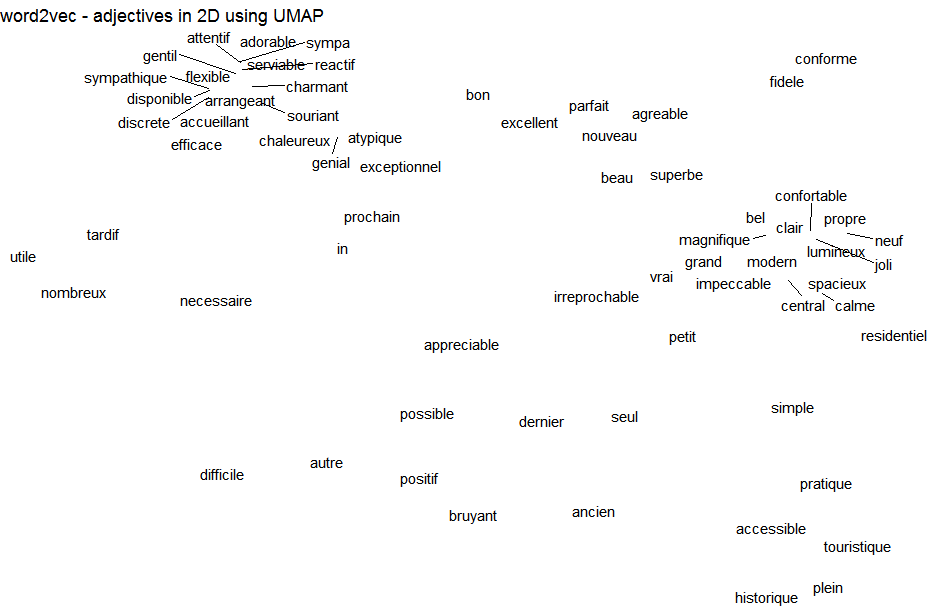
\includegraphics[width=0.6\textwidth]{informatica/word2vec_example}
        \caption{Ejemplo de un \textit{embedding} semántico, computado por el modelo \textit{word2vec} \cite{informatica:word2vec}, de palabras en francés. Imagen extraída de \cite{informatica:word2vec_cran_package}}
    \end{figure}

    En el caso concreto de \cite{informatica:word2vec}, que propone el conocido modelo \textit{word2vec}, se consigue que el \textit{embedding} tenga cierta \entrecomillado{estructura algebraica}, pudiendo computar, por ejemplo:

    \begin{equation}
        vector("rey") - vector("hombre") + vector("mujer") = vector("reina")
    \end{equation}
\end{ejemplo}

\begin{ejemplo}
    Veamos ahora un ejemplo mucho más cercano con el problema que queremos resolver. Por ejemplo, el problema de re-identificación (ambiente en el que se proponen las nuevas técnicas de cómputo del \textit{triplet loss} \cite{informatica:principal}).

    En este caso, queremos que las imágenes de una persona en una escena, se transformen a vectores cercanos, como muestra la siguiente representación:

    \begin{figure}[H]
        \centering
        \includegraphics[width=0.6\textwidth]{informatica/embedding_paper_principal}
        \caption{Imagen extraída de \cite{informatica:principal}. Se representa una porción del \textit{dataset} \textit{Market-1501} tras aplicar el \textit{embedding} aprendido y posteriormente \textit{t-SNE}}
    \end{figure}

    Por ejemplo, un modelo que quiera resolver esta tarea podría aprender a mapear personas con exactamente la misma ropa a puntos cercanos.
\end{ejemplo}

\begin{ejemplo}

    Y para finalizar, consideremos nuestra tarea en concreto. Buscamos que las imágenes de la misma persona, aunque hayan pasado los años, se transformen en vectores cercanos. Y al contrario, que imágenes de dos personas distintas estén lo más lejos posible.

    Esto es especialmente complicado, como ya hemos comentando en \customref{ich:descrp_problema}, porque por ejemplo, nuestro modelo debe ver como más cercanos imágenes de un niño y un adulto con barba (ambos siendo la misma persona) que dos imágenes de dos adultos con barba (siendo distintas personas). Este problema en concreto lo hemos mostrado en \customref{img:messi_distintos_otro_adulto}

\end{ejemplo}

\section{\textit{Triplet Loss}} \label{isec:triplet_loss}

Nuestro objetivo es ahora justificar el uso de \textit{triplet loss} como una función de pérdida que permita a nuestro modelo aprender un \textit{embedding} semántico.

Recordemos que estamos trabajando con funciones de la forma:

\begin{equation}
\begin{split}
    f_{\theta}: X & \to \R^N \\
    x & \mapsto f_{\theta}(x)
\end{split}
\end{equation}

y con una métrica:

\begin{equation}
\begin{split}
    D: X \times X & \to [0, \infty) \\
    x, y & \mapsto D(x, y)
\end{split}
\end{equation}

Para ser más concisos, usaremos la notación $D_{i, j} := D(f_{\theta}(x_i), f_{\theta}(x_j))$.

Como su nombre indica, \textit{triplet loss} trabajará sobre triples. Esto es:

\begin{enumerate}
    \item Una imagen de un individuo concreto, a la que llamaremos \textbf{\textit{anchor}} o ancla
    \item Otra imagen distinta, pero del mismo individuo, a la que llamaremos \textbf{positiva}
    \item Una imagen de un individuo distinto, a la que llamaremos \textbf{negativa}
\end{enumerate}

En este caso, queremos que la distancia entre el \textit{embedding} del ancla y el \textit{embedding} de la positiva (que podemos denotar como $D_{A, P}$) sea mucho menor que la distancia entre el \textit{embedding} del ancla y el \textit{embedding} de la negativa (denotamos $D_{A, N}$). Por tanto, lo que realmente queremos es que:

\begin{equation}
    D_{A, P} \leq D_{A, N}
\end{equation}

o lo que es lo mismo,

\begin{equation}
    D_{A, P} - D_{A, N} \leq 0
\end{equation}

Una forma trivial de hacer que esa ecuación se cumpla, es haciendo que

\begin{equation}
    f(x) = \vec{0}; \dspace \forall x \in X
\end{equation}

con lo que obtendríamos un modelo totalmente inservible. Para evitar eso, introducimos un término $\alpha > 0$ que se conoce como \textbf{margen}, llegando a:

\begin{equation}
    D_{A, P} - D_{A, N} + \alpha \leq 0
\end{equation}

Buscamos que el término de la izquierda sea lo más negativo posible, por lo buscamos minimizar la siguiente función de pérdida:

\begin{equation} \label{ieq:triplet_loss_single_entry}
\begin{split}
    \mathcal{L}_{tri}(\theta; A, P, N) & := max \{D_{A, P} - D_{A, N} + \alpha, 0 \} = \ldots \\
    \ldots &= ReLU(D_{A, P} - D_{A, N} + \alpha)
\end{split}
\end{equation}

Minimizando esta función de pérdida, lo que haremos será atraer elementos de la misma clase entre sí, y alejar elementos de clases distintas. Este proceso se refleja en la siguiente imagen:

\begin{figure}[H]
    \centering
    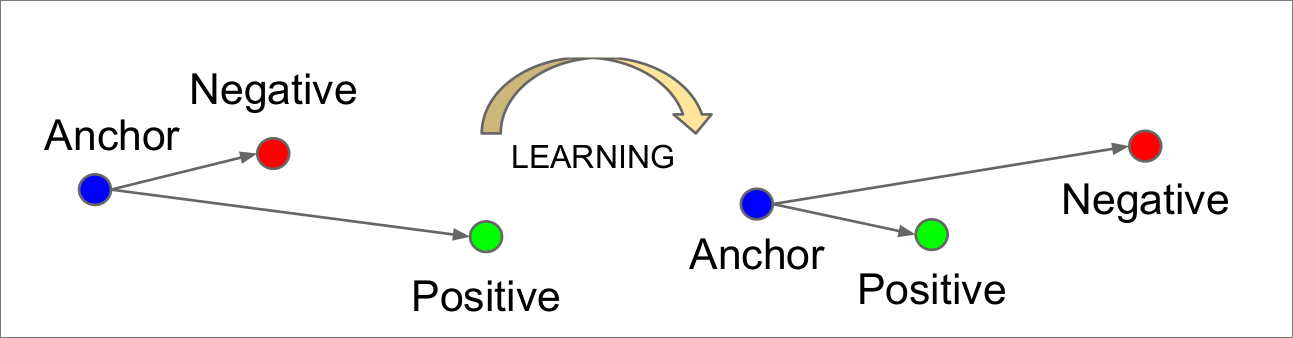
\includegraphics[width=0.8\textwidth]{informatica/triplet_loss_learning}
    \caption{Ejemplo gráfico del proceso de aprendizaje deseado con \textit{triplet loss}. Imagen extraída de \cite{informatica:facenet}}
\end{figure}

Sin embargo, en \eqref{ieq:triplet_loss_single_entry} trabajamos con una sola entrada de tres datos. A diferencia de un \textit{dataset} con datos etiquetados clásico, de la forma \lstinline{(entrada, valor de etiqueta)}, tenemos datos de la forma \lstinline{(imagen, identificador de individuo, edad)}. Esto supone un \textbf{problema} a resolver: cómo generamos \textit{batches} con triples de la forma \lstinline{(ancla, positivo, negativo)} para poder aplicar \eqref{ieq:triplet_loss_single_entry}. Introducimos algunas soluciones propuestas a este problema en \customref{isec:batching}

Por otro lado, este enfoque plantea algunas \textbf{ventajas}. La principal es que, a diferencia de otros enfoques basados en usar funciones de pérdida auxiliares (y que suelen fuerzan que la red solo pueda funcionar comparando pares de imágenes), el cómputo del \textit{embedding} es directo usando esta función de pérdida (\textit{end to end learning}). Optimizamos directamente la propiedad semántica del \textit{embedding} que deseamos obtener. Una vez entrenado el modelo es directo adaptar el modelo a tareas de \textit{clustering}, \textit{retrieval}, verificación, \ldots \cite{informatica:principal}. En \customref{isubs:impl_retr_adapter}, mostramos cómo podemos realizar una de estas adaptaciones.

\section{Generación de \textit{batches}} \label{isec:batching}

Como ya hemos comentado, la tarea que debemos resolver ahora es la de generación de \textit{batches} adecuados para poder emplear \eqref{ieq:triplet_loss_single_entry} como función de pérdida a minimizar.

Por tanto, dado un conjunto de datos de la forma \lstinline{(imagen, identificador, edad)}, debemos obtener un conjunto de datos de la forma \lstinline{(img. ancla, img. positivo, img. negativo)}. Este último conjunto de datos puede ser una lista de triples o un conjunto de \textit{batches}. Como buscamos trabajar con \textit{batches}, en el caso de tener una lista de triples, podemos simplemente muestrear aleatoriamente y sin remplazo de dicha lista, repitiendo el muestreo tras cada época completada.

\subsection{Enfoque \textit{offline}} \label{isubs:enfoque_offline_minado_triples}

Este es el enfoque clásico que se ha venido usando previo a \cite{informatica:facenet}, trabajo que introduce un enfoque \textit{online} que luego otros trabajos como \cite{informatica:principal} han ido mejorando.

En este enfoque, el ciclo de aprendizaje se divide en \textbf{varios pasos}.

En primer lugar, se realiza un \textbf{minado \textit{offline}} de los triples. Es decir, se obtiene una primera lista o conjunto de \textit{batches} de la forma \lstinline{(img. ancla, img.positivo, img.negativo)}. Una forma de hacer esto sería, por ejemplo, generar los triples de forma aleatoria, generar todos los posibles triples, $\ldots\dspace$ Aunque estas ideas no suelen funcionar en la práctica. Otra forma más efectiva es seleccionar los triples en base a algún estudio estadístico. O usar la red que vamos a optimizar para identificar aquellos triples en los que tiene más dificultad.

En segundo lugar, realizamos el aprendizaje sobre dicho conjunto de triples. En algunos casos, realizamos el entrenamiento completo sobre dicho conjunto inicial. En otros casos, principalmente cuando usamos la red para el minado de triples, pasadas algunas épocas de entrenamiento volvemos a generar otra vez la lista de triples. Así, triples que antes la red no identificaba propiamente, ahora sí que los identifica (\entrecomillado{network snapshots}, \cite{informatica:facenet}) y podemos buscar triples más interesantes.

Una vez computado una lista de triples $(a, p, n) \in \Omega$, la función de pérdida \eqref{ieq:triplet_loss_single_entry} se implementa de forma natural como en cualquier otro ámbito de \textit{batching}:

\begin{equation}
    \mathcal{L}_{tri}^{offline}(\theta; \Omega) := \frac{1}{\#\Omega} \sum_{(a, p, n) \in \Omega} \mathcal{L}_{tri}(\theta; a, p, n)
\end{equation}

\begin{observacion}

En la literatura sobre aprendizaje automático normalmente se ignora el término $\frac{1}{\#\Omega}$ y se supone que siempre estamos dividiendo por el número de sumandos, con lo que nuestra función de error suele escribirse como:

\begin{equation}
    \mathcal{L}_{tri}^{offline}(\theta; \Omega) := \sum_{(a, p, n) \in \Omega} \mathcal{L}_{tri}(\theta; a, p, n)
\end{equation}


\end{observacion}

Este enfoque supone una serie de \textbf{problemas}:

\begin{itemize}
    \item Estamos dividiendo el proceso de aprendizaje en dos etapas, la de minado de triples y la de aprendizaje sobre estos triples. Esto añade complejidad a nuestra \textit{pipeline} (véase \customref{isec:pipeline})
    \item La adecuada elección de triples es fundamental. Si elegimos triples demasiado fáciles, la red no aprenderá nada nuevo, pues es muy fácil distinguir los ejemplos presentados. Sin embargo, si solo mostramos triples complicados, el modelo se centrará en aprender ejemplos extraordinarios y no sabrá distinguir el grueso de ejemplos más sencillos
        \begin{itemize}
            \item Además, generalmente los modelos aprenden rápidamente a distinguir la mayoría de ejemplos en los que las diferencias son relativamente evidentes. Por tanto, en pocas iteraciones la mayoría de triples generados de forma \textit{offline} son demasiado sencillos, lo que agrava mucho el problema que hemos comentado
        \end{itemize}
    \item Sería conveniente disponer de alguna forma de ajustar la complejidad de los triples presentados. Podemos confiar en que al ir re-generando la lista de triples, la complejidad vaya aumentando. Pero el algoritmo de minado debería tener alguna forma de controlar el énfasis que se hace en la búsqueda de combinaciones difíciles, lo que añade aún más complejidad al sistema
    \item El minado supone realizar un proceso de búsqueda, que es \textbf{muy lento} (evaluar de alguna forma todos los posibles triples supondría al menos $O(n^3)$). Lo ideal sería disponer de algún método que se basará en muestrear aleatoriamente de nuestra lista de elementos de la forma \lstinline{(imagen, identidad, edad)} (proceso que es muy rápido) y generar triples interesantes sobre dicho muestreo. Esto motiva la técnica introducida en \customref{isubs:triples_online}
\end{itemize}

\subsection{Enfoque \textit{online}} \label{isubs:triples_online}

La idea común será la de implementar el siguiente proceso. En primer lugar, realizaremos un muestreo aleatorio sobre los datos de la forma \lstinline{(imagen, identidad, edad)}. Este muestreo es rápido y no supone prácticamente tiempo de cómputo. Usando únicamente los datos de ese muestreo, generaremos triples y computaremos la función de pérdida apoyándonos en \eqref{ieq:triplet_loss_single_entry}. Dicha generación ya sí que supone un tiempo de cómputo considerable. Repetimos este proceso hasta agotar todos las entradas de nuestro \textit{dataset}, completando así una época de entrenamiento.

Ya podemos ver algunas \textbf{ventajas de este método}, incluso antes de haber especificado las dos partes fundamentales del proceso (muestreo y selección de triples):

\begin{enumerate}
    \item La ventaja más obvia es que, suponiendo que el tamaño de la muestra es significativamente mucho más pequeño que el tamaño de todo el conjunto de datos, la generación de triples consumirá potencialmente menos tiempo y será más efectiva
        \begin{itemize}
            \item Para afirmar esto rotundamente, tendríamos que realizar un estudio del tiempo del minado \textit{offline} en contraste a la suma de todos los tiempos de minado en cada muestreo
            \item Sin embargo, el tiempo usado es más eficiente, porque en cada muestreo estamos usando la red actualizada. En el minado \textit{offline} podemos gastar muchísimo tiempo en encontrar triples difíciles que, tras entrenar en unos pocos triples previos, acaben siendo sencillos. Por tanto, cuando la red vea triples algo avanzados en la lista, estos ya serán totalmente inútiles
        \end{itemize}
    \item Se facilita en gran parte el ajuste de la dificultad. Podemos buscar triples realmente difíciles, pero como solo se tiene acceso a una pequeña muestra, estamos controlando la dificultad. Así que podemos variar el tamaño de las muestras para buscar un punto medio entre ejemplos muy difíciles o ejemplos demasiado sencillos. Y todo esto sin contar con el factor de que vamos a usar la red actualizada para la elección de los triples
\end{enumerate}

Desarrollada esta visión de forma general, veamos cómo se implementa cada una de las partes, siguiendo las técnicas introducidas en \cite{informatica:principal}.

\subsection{Muestreo de los datos con \textit{P-K sampling}} \label{isubs:muestreo_datos_pk_sampling_teoria}

La \textbf{idea principal del muestreo} es lo que definiremos como \textbf{\textit{P-K sampling}}. Como ya hemos comentado en \customref{isubs:triples_online}, nuestra tarea ahora es generar un \textit{batch} de elementos de la forma \lstinline{(imagen, identidad, edad)}. En una segunda etapa (véase \customref{isubs:seleccion_de_triples}), otro algoritmo decide cómo generar triples a partir de estos datos.

El algoritmo de muestreo \textit{P-K sampling} es muy sencillo. En cada muestreo, seleccionamos aleatoriamente $P$ identidades de individuos (o clases, en un ambiente más general en el que no necesariamente estemos trabajando con imágenes de personas). Por cada una de las identidades, seleccionamos aleatoriamente $K$ imágenes asociadas a esa identidad. Por tanto, obtenemos una lista de $P \cdot K$ imágenes, a la que llamaremos \textbf{\textit{P-K batch}}. Para poder obtener triples interesantes en la siguiente etapa, parece que lo deseable es que ambos muestreos aleatorios sean sin repetición.

El hecho de tener $K$ imágenes por cada uno de los individuos seleccionados es lo que va a permitir al algoritmo de generación de triples obtener rápidamente triples interesantes.

\begin{figure}[H]
    \centering
    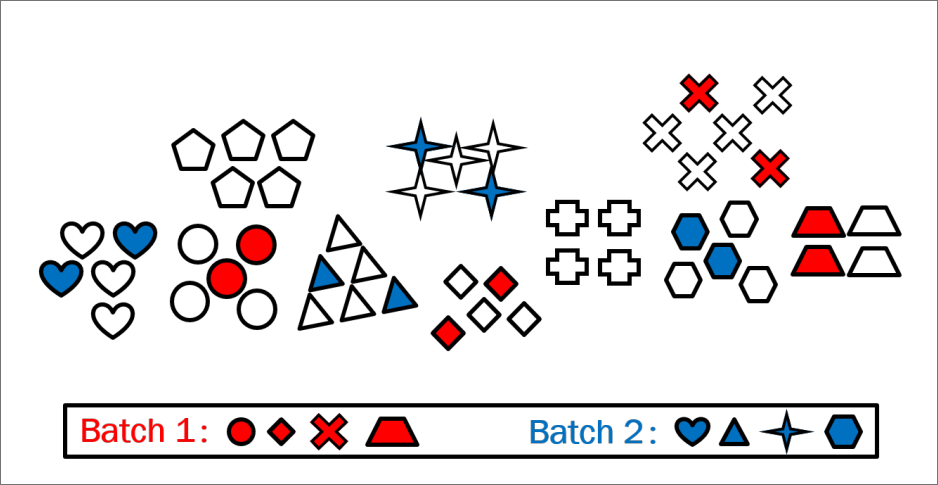
\includegraphics[width=0.6\textwidth]{informatica/ejemplo_grafico_pk_sampling}
    \caption{Ejemplo gráfico del proceso de \textit{P-K sampling}. Imagen extraída de \cite{informatica:paper_image_pk_sampling}}
\end{figure}

Queda aquí claro el \textbf{problema principal} que introduce esta técnica: si queremos muestrear $K$ imágenes de cada individuo sin repetición, cada individuo debe tener asociadas al menos $K$ imágenes. Así que a la hora de trabajar con un \textit{dataset}, siempre deberíamos comprobar la distribución del número de imágenes por individuo, como haremos en \customref{isec:base_datos_usada}.

\subsection{Selección de triples y funciones de pérdida} \label{isubs:seleccion_de_triples}

Una vez que tenemos un \textit{batch} de $P \cdot K$ elementos, deberemos generar una lista de triples en base a este \textit{batch}. Una vez se especifica cómo se seleccionan los triples, usando \eqref{ieq:triplet_loss_single_entry}, inducimos de forma natural y directa una cierta función de pérdida que actúa sobre estos \textit{P-K batches}.

\begin{observacion}[Notación para los \textit{P-K batches}] \label{iobs:notacion_pk_formulas}

    Vamos a trabajar con $P \cdot K$ elementos, cada uno correspondiendo a una clase en concreto. Por tanto, indexaremos los elementos de la forma $x_k^p$ donde $p$ marca el identificador del individuo, y $k$ marca a cuál de las $K$ imágenes del individuo $p$ nos estamos refiriendo

\end{observacion}

\subsubsection{\textit{Batch Hard}} \label{isubsubs:batch_hard}

La primera idea es iterar sobre todos los elementos del \textit{P-K batch}, obteniendo así $P \cdot K$ anclas. Por cada ancla, seleccionamos el positivo y negativo \textbf{más complicado dentro de \textit{P-K batch}}. Por tanto, queda claro que \textbf{estamos usando la red para seleccionar triples difíciles} en cada \textit{batch} generado.

Esto introduce la siguiente función de pérdida, a la que llamaremos \textbf{\textit{Batch Hard}}:

\begin{equation}
    \mathcal{L}_{BH}(\theta, \hat{\Omega}) := \comentarencima{\sum_{p = 1}^P \sum_{k = 1}^K}{\text{todas las anclas}} [
        \comentarencima{\max_{k' = 1, \ldots, K} D(f_{\theta}(x_k^p), f_{\theta}(x_{k'}^p))}{\text{positivo más complicado}}
        - \comentarencima{\min_{\substack{p' = 1, \ldots, P \\ p' \neq p \\ k' = 1, \ldots, K}} D(f_{\theta}(x_k^p), f_{\theta}(x_{k'}^{p'}))}{\text{negativo más complicado}}
        + \alpha]_+
\end{equation}

donde $[x]_+ := max \{0, x\} = ReLU(x)$ y $\hat{\Omega}$ se refiere a un \textit{P-K batch}. No olvidemos que no estamos escribiendo la división por el número de sumandos, $P \cdot K$.

Estamos generando \textbf{triples moderados}, porque estamos buscando los triples más difíciles, pero dentro de un \textit{batch} relativamente pequeño comparado a el total del conjunto de datos. Con esto estamos ajustando la dificultad de los triples cómodamente, resolviendo el problema que comentábamos en \customref{isubs:enfoque_offline_minado_triples}. Aumentando el valor de $\{P, K\}$ aumentamos el tamaño del espacio de búsqueda, y por tanto podremos encontrar triples mucho más difíciles. Sin embargo, hay que tener siempre en cuenta el coste en tiempo de cómputo.

Queda claro que, gracias al proceso de \textit{P-K sampling}, ahora es factible realizar una búsqueda de triples interesantes en profundidad, basándonos en el estado más actualizado de la red para calcular la dificultad de los triples. Esta búsqueda extensiva no habría sido posible si la planteásemos sobre todo el conjunto de datos.

\subsubsection{\textit{Batch All}} \label{isubsubs:batch_all}

Motivados por lo que acabamos de comentar en \customref{isubsubs:batch_hard}, podemos plantearnos usar todos los posibles triples dentro de un \textit{P-K batch} como un enfoque que ahora cobra más sentido (ya hemos comentado en \customref{isubs:enfoque_offline_minado_triples} que realizar esto sobre todo el conjunto de datos no parece una buena idea).

Realizar esto introduce la función de pérdida que llamaremos \textbf{\textit{Batch All}}:

\begin{equation} \label{ieq:batch_all}
    \mathcal{L}_{BA}(\theta; \hat{\Omega}) :=
    \comentarencima{\sum_{p = 1}^{P} \sum_{k = 1}^K}{\text{todas anclas}}
    \comentardebajo{\sum_{\substack{k' = 1 \\ k' \neq k}}^{K}}{\text{todas pos.}}
    \comentarencima{\sum_{\substack{p' = 1 \\ p' \neq p}}^P \sum_{n = 1}^K}{\text{todas neg.}} \dspace[
        D(f_{\theta}(x_k^p),f_{\theta}(x_{k'}^p)) - D(f_{\theta}(x_k^p),f_{\theta}(x_{n}^{p'})) + \alpha
    ]_+
\end{equation}

Está claro que, por el número de sumandos, esta aproximación es viable gracias a que nuestro \textit{P-K sampling} reduce mucho el número de elementos sobre los que operamos. Dicho número de sumandos viene dado por:

\begin{equation}
    P \cdot K \cdot (K - 1) \cdot (P - 1) \cdot K = P^2 - P + K^3 - K^2 \approx P^2 + K^3
\end{equation}

Esta aproximación sería completamente inviable sobre un número muy elevado de elementos. Pensemos, por ejemplo, en las 163446 imágenes de \textit{CACD} (véase \customref{isec:dataset_cacd}).

\subsubsection{Mejoras introducidas a partir de la experimentación} \label{isubsubs:mejoras_sumandos_no_nulos}

En \cite{informatica:principal}, a raíz de observar los resultados de la experimentación, señalan algunos puntos débiles en las dos funciones de pérdida que introducen a partir del \textit{P-K sampling}.

Principalmente, en \customref{isubsubs:batch_all}, podemos ver un posible fallo en la función de pérdida \eqref{ieq:batch_all}. Si se da el caso de que la mayoría de triples generados son fáciles (hecho muy probable al estar generando todas las combinaciones de triples), los escasos triples que realmente son difíciles se desvanecerán. Esto porque la mayoría de términos serán cero (al estar aplicando $[x]_+$). Y los pocos términos que no son cero, se dividen por el número total de elementos, que ya hemos visto que es elevado.

Por tanto, una mejora sencilla a esta función de pérdida es dividir únicamente por el número de sumandos no nulos. A estos sumandos no nulos también se les llama sumandos activos \cite{informatica:principal}. Esta mejora la podemos aplicar también a \textit{batch hard}, obteniendo dos nuevas funciones de pérdida, a las que denotaremos por $\mathcal{L}_{BA \neq 0}$ y $\mathcal{L}_{BH \neq 0}$.

\subsubsection{Algunas observaciones y conclusiones} \label{isubsubs:observaciones_conclusiones_pksampling}

En primer lugar, cabe destacar que, como señalan \cite{informatica:principal}, las dos nuevas funciones de pérdida introducidas equivalen al planteamiento clásico de \textit{triplet loss} si entrenásemos indefinidamente.

El desarrollo que hemos realizado justifica las siguientes \textbf{ventajas} de los nuevos métodos:

\begin{itemize}
    \item El uso del \textit{P-K sampling} y las dos nuevas funciones de pérdida (con las variantes técnicas que consideran los sumandos activos) permite realizar un aprendizaje \textit{end-to-end}, sin añadir un paso adicional en el bucle de aprendizaje, evitando así la gran complejidad añadida del minado \textit{offline}
    \item Además, conseguimos un manejo preciso de la dificultad de los triples obtenidos. Controlando el valor de $\{P, K\}$, controlamos el espacio de búsqueda y, en definitiva, la dificultad. Todo esto de forma cómoda y sin introducir apenas complejidad en nuestro \textit{pipeline}
    \item Aunque no lo hemos comprobado, pensamos que esto acelera los tiempos de cómputo, al estar realizando el minado de triples sobre \textit{batches} de tamaño considerablemente reducidos
    \item Y aunque no mejorásemos el tiempo de computo, lo que sí sabemos que mejoramos es la eficacia del minado de triples. El minado de triples \textit{online} usa una red mucho más actualizada, para generar una lista mucho más pequeña que probablemente no se degrade tanto como la generada por un minado \textit{offline} sobre todo el conjunto de datos, mucho más grande
    \item Es más, estamos controlando el efecto de los triples demasiado sencillos, que no tendremos en cuenta a la hora de promediar en la función de pérdida
\end{itemize}

A pesar de esto, a raíz de trabajar con estas nuevas técnicas, identificamos los siguientes \textbf{inconvenientes}:

\begin{itemize}
    \item Introducimos dos hiperparámetros, $\{P, K\}$ que deberemos ajustar correctamente, pues tienen un enorme impacto en los resultados del proceso de entrenamiento. Por tanto, se hace fundamental tener un proceso de \textit{hyperparameter tuning} robusto, como introducimos en \customref{isec:hptuning_kfold_cross_validation} e implementamos en \customref{isec:hp_tuning}
    \item Tenemos que tener mucho cuidado con usar valores elevados de $\{P, K\}$ por dos motivos. El primero, y como ya hemos comentado, valores altos implicarán que los tiempos de cómputo para la generación de triples crecerán rápidamente. El segundo es que el tamaño de los \textit{batches} crecerán considerablemente, llegando a colapsar la memoria disponible de la \textit{GPU}
    \item Hemos comprobado en la práctica que es realmente fácil colapsar la memoria \textit{GPU}, usando modelos profundos como \textit{ResNet50} con valores de $P \cdot K = 100$. Esto supone que, aunque no estuviéramos limitados por el tiempo de cómputo, el colapso de la memoria limita el conjunto de valores $\{P, K\}$ con los que podemos experimentar
    \item Si queremos usar valores altos de $K$, nuestro \textit{dataset} lo debe permitir, teniendo una buena distribución de imágenes por individuo. Por este motivo hemos estudiado esta distribución en \customref{isec:base_datos_usada}. Se pueden explorar técnicas como el aumentado de datos para alcanzar el número de imágenes por individuo deseado, pero solo serán efectivas si dicha distribución es buena para empezar (véase \customref{isec:aumentado_datos})
    \item Tanto por el formato de los datos con los que hemos trabajado, como por el cambio fundamental realizado en el \textit{sampling} de los datos, hemos tenido que realizar un \textbf{esfuerzo considerable de implementación}, al no poder basarnos en la mayor parte de los casos en código implementado por alguna biblioteca de aprendizaje automático. Esto se ve reflejado en \customref{ich:implementacion}
\end{itemize}

\section{Función de distancia}

En todos los conceptos que hemos ido introduciendo la función de distancia


\begin{equation}
    D: X \times X \to [0, \infty)
\end{equation}

ha estado presente, pero todavía no hemos introducido ninguna función concreta. En el ambiente de \textit{AIFR} se suele usar la distancia euclídea al cuadrado, esto es:

\begin{equation}
    D(x_i, x_j) := ||f_{\theta}(x_i) - f_{\theta}(x_j)||^2_2
\end{equation}

Sin embargo, motivados por \cite{informatica:principal}, decidimos usar la distancia euclídea usual. En este trabajo se afirma que, en base a la experimentación, de esta forma se obtienen entrenamientos más estables. Además, usando la distancia euclídea usual, el margen es más fácil de interpretar, porque marca la diferencia de distancias, y no la diferencia de cuadrados de distancias. Por lo tanto, en base a dicho trabajo, decidimos tomar:

\begin{equation}
        D(x_i, x_j) := ||f_{\theta}(x_i) - f_{\theta}(x_j)||_2
\end{equation}

\section{Márgenes suaves} \label{isec:margenes_suaves}

En \customref{isec:triplet_loss} hemos justificado por qué es necesario introducir un término $\alpha$ para controlar el margen y evitar que nuestro modelo aprenda a colapsar todas las entradas al vector $\vec{0}$. Con esto llegamos a la ecuación \eqref{ieq:triplet_loss_single_entry}.

En dicha función de pérdida, el propósito de $x \mapsto \max\{0, x + \alpha\}$ (conocida comúnmente como \textit{hinge function} \cite{informatica:principal}) es no corregir ejemplos que, en vista del margen $\alpha$ establecido, ya son correctos. Pero puede ser que estemos interesados en afinar aún más ejemplos que, para dicho valor del margen, sean correctos. Con esto conseguiríamos seguir acercando imágenes del mismo individuo lo máximo posible \cite{informatica:principal}.

Es por esto que se propone en \cite{informatica:principal} usar la función \textbf{\textit{softplus}}:

\begin{equation}
    x \mapsto ln(1 + exp(x))
\end{equation}

Dicha función puede verse como una versión suavizada de la función \textit{hinge}. Decae exponencialmente, por lo que ejemplos correctos se penalizarán exponencialmente menos cuanto más cercanos estén, pero contrasta con la función \textit{hinge} en que no presenta un salto o corte fuerte. Por tanto, se suele decir que estamos usando un \textbf{margen suave}.

Además, una ventaja de esta función es que \textbf{desechamos el hiperparámetro $\alpha$}, el cual ya no tenemos que fijar a través de algún método (como podría ser el \textit{hyperparameter tuning}).

\begin{figure}[H]
\centering
    \begin{subfigure}{.5\textwidth}
        \centering
        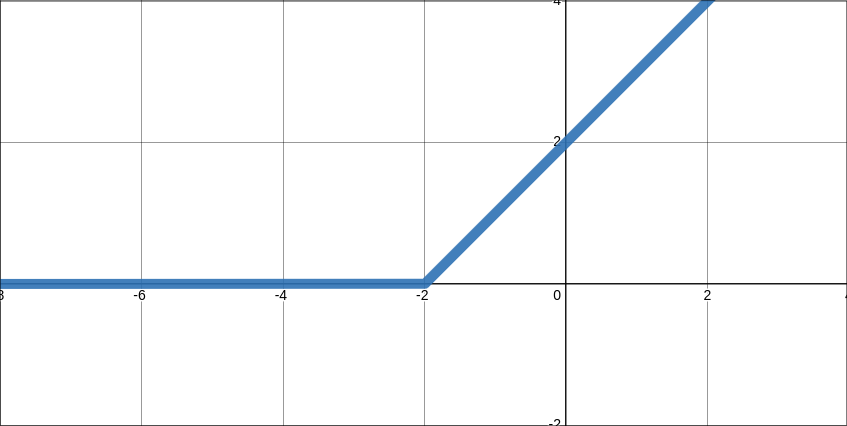
\includegraphics[width=0.8\linewidth]{informatica/desmos_hinge}
        \caption{Función \textit{hinge} con $\alpha = 2$}
    \end{subfigure}%
    \begin{subfigure}{.5\textwidth}
        \centering
        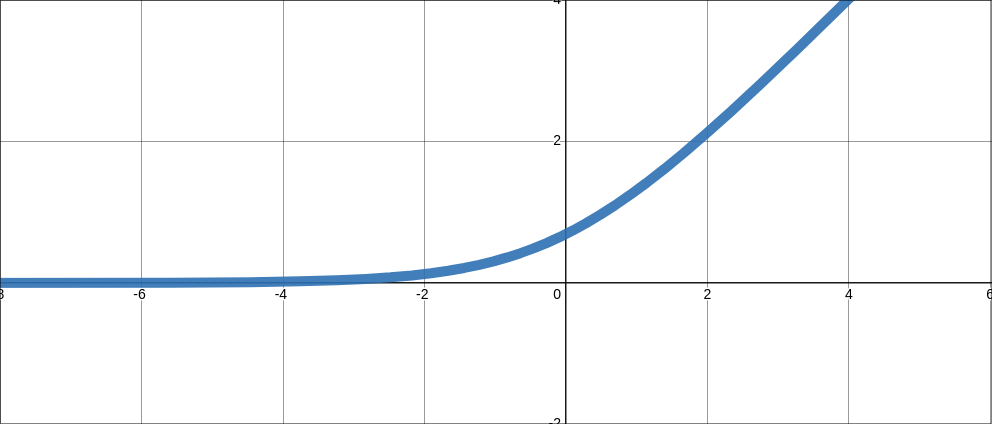
\includegraphics[width=0.8\linewidth]{informatica/desmos_softplus}
        \caption{Función \textit{softplus}}
    \end{subfigure}

    \begin{subfigure}{.5\textwidth}
        \centering
        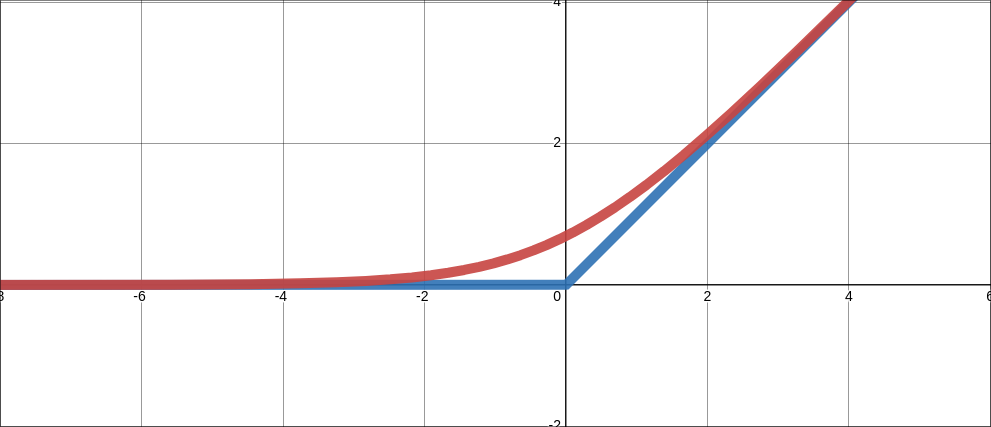
\includegraphics[width=0.8\linewidth]{informatica/desmos_conjunta}
        \caption{En azul, \textit{hinge} con $alpha = 0$. En rojo, \textit{softplus}}
    \end{subfigure}


\caption{Gráfica de las dos funciones para trabajar con los márgenes, y una gráfica conjunta que muestra su similitud}
    \label{img:graficas_margenes}
\end{figure}

Las gráficas mostradas en \customref{img:graficas_margenes} nos sirven para visualizar de forma sencilla todo lo que hemos comentado. La función \textit{softplus} actúa como una \textit{hinge} suavizada. El hecho de que se parezcan tanto cuando hacemos que el margen de \textit{hinge} sea cero nos hace pensar que \textit{softplus} va a actuar como una \textit{hinge} en la que no hay margen, y por lo tanto, acercará elementos de la misma clase todo lo que pueda.

